\chapter{Results}
\label{chap:results}

\section{YOLO Results}
\label{sec:training-results}
This section presents the performance of the YOLO26n and YOLO26m model for vehicle detection and classification, and provides the empirical basis for assessing the first research question. For YOLO26n, the training process was conducted for 87 epochs, at which point early stopping was triggered as the validation loss reached a plateau. YOLO26m finished all 100 epochs. The following results are evaluated based on both the validation dataset used during training and an independent test set to ensure the model's generalizability to unseen data. The train/val/test split is identical for both model sizes.

\subsection{Training and Validation}
\label{sec:yolo_train_val}
\subsubsection*{mAP$^{50-95}$ and mAP$^{50}$}
The training progress of the YOLO26n and YOLO26m models was evaluated using mAP$^{50-95}$ and mAP$^{50}$. As shown in \autoref{fig:train_val_map}, both models exhibit a consistent upward trajectory. The YOLO26m model achieves a higher peak mAP$^{50}$ of 0.9027, compared to 0.7421 for the YOLO26n variant. Similarly, for the stricter mAP$^{50-95}$ metric, YOLO26m reaches a peak of 0.7237, while YOLO26n peaks at 0.5989. Performance for both models effectively plateaus after epoch 55, indicating they have reached their learning capacity for the dataset.

\begin{figure}[H]
\centering
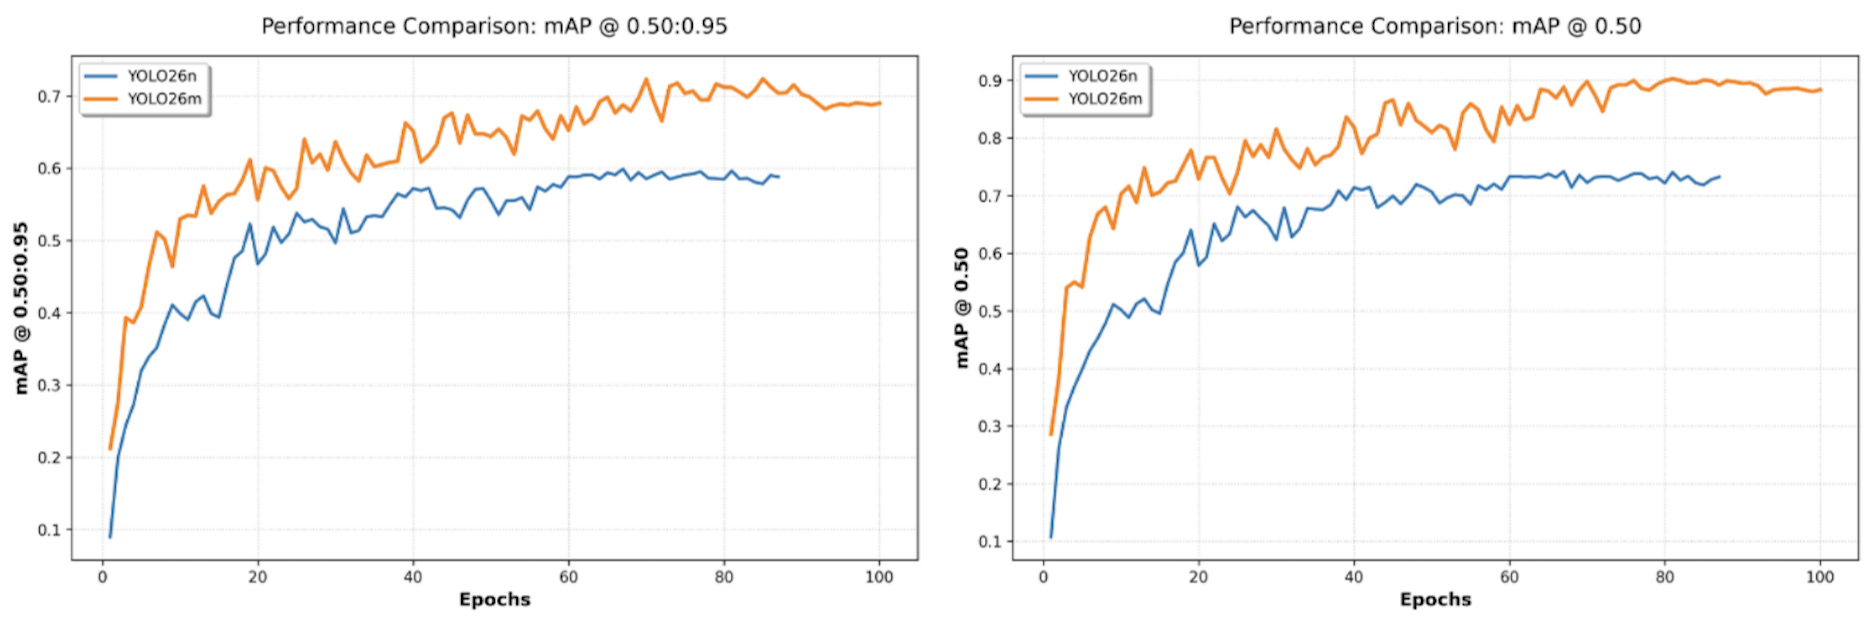
\includegraphics[width=1.0\linewidth]{project/images/yolo_n_vs_m/train_val_map.png}
\caption{Training progress comparison of YOLO26n and YOLO26m for mAP$^{50-95}$ (left) and mAP$^{50}$ (right).}
\label{fig:train_val_map}
\end{figure}

\subsubsection*{Precision and Recall}
The specific trade-offs between Precision and Recall are illustrated in \autoref{fig:train_val_pr}. While both metrics maintain a general upward trend, they exhibit higher volatility compared to the mAP scores. The YOLO26m variant demonstrates significantly superior sensitivity, reaching a peak recall of 0.8658, whereas YOLO26n reaches a maximum of 0.7085. In terms of Precision, YOLO26m peaks at 0.9239 and YOLO26n at 0.9083. Although Precision shows sharp fluctuations between epochs 10 and 50, both models stabilize in the later stages of training, ensuring reliable vehicle detection.

\begin{figure}[H]
\centering
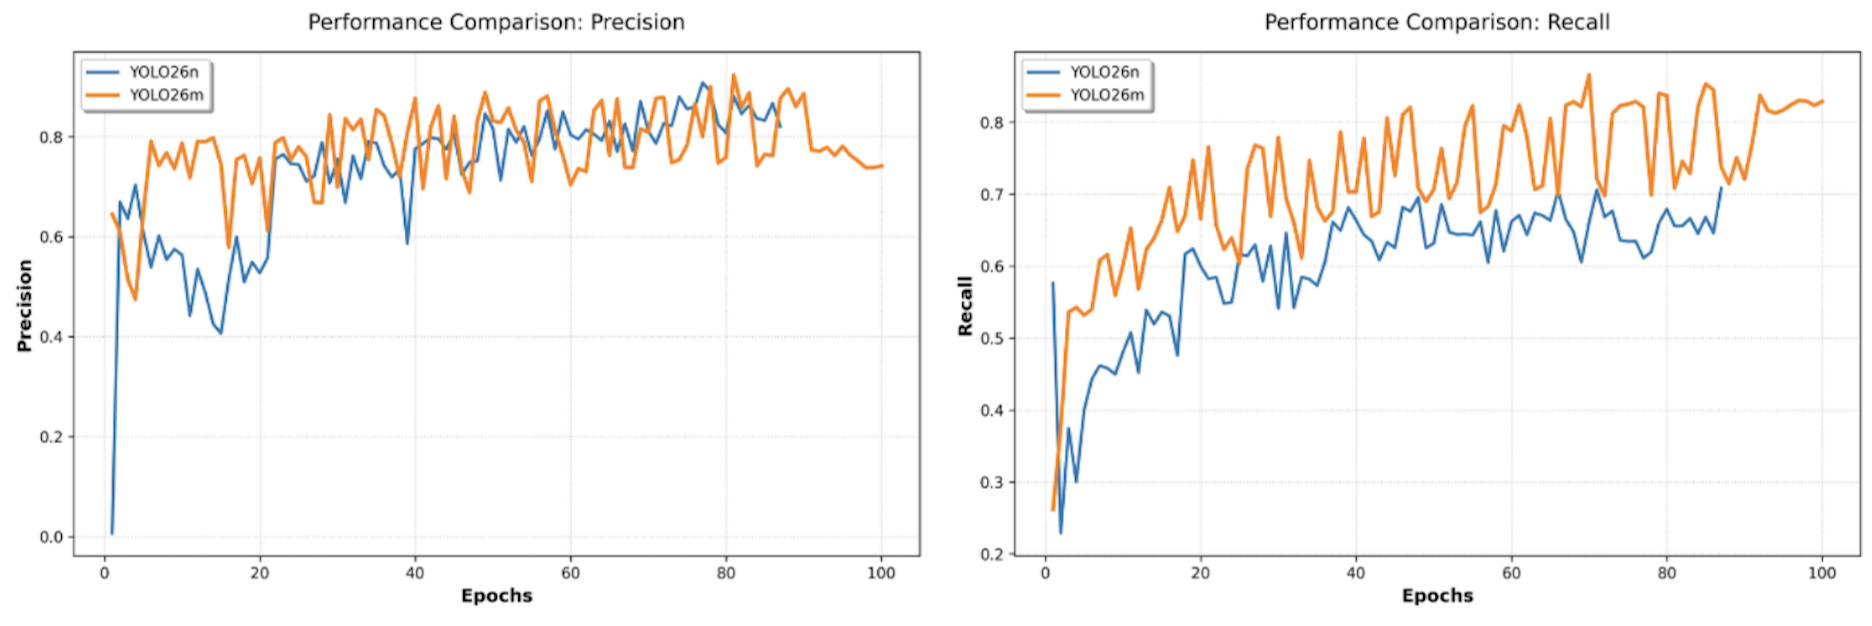
\includegraphics[width=1.0\linewidth]{project/images/yolo_n_vs_m/train_val_pr.png}
\caption{Training progress comparison of YOLO26n and YOLO26m for Precision (left) and Recall (right).}
\label{fig:train_val_pr}
\end{figure}

For a more comprehensive overview of the model’s training and validation, validation set results are presented in Appendix \ref{app:raw_metrics}. 



\subsection{Performance on Test Set}
\label{sec:test_results}
The final performance of both the YOLO26n and YOLO26m models was evaluated on the same independent test set of 193 images containing 761 object instances, as detailed in \autoref{tab:test_results_n} and \autoref{tab:test_results_m}. The YOLO26n model achieved an overall mAP$^{50}$ of 0.693 and an mAP$^{50-95}$ of 0.556, while the YOLO26m variant delivered noticeably stronger results with an mAP$^{50}$ of 0.808 and an mAP$^{50-95}$ of 0.638. Notably, the validation metrics were even stronger.

Analysis of individual classes shows that the ’Car’ category remains the most accurately detected for both models, with AP$^{50}$ values of 0.945 (YOLO26n) and 0.960 (YOLO26m) and recall values above 0.91. Large vehicle categories such as ’Heavy Truck’ and ’Semi-trailer’ also demonstrated high reliability across both variants (mAP$^{50}$ of 0.743/0.817 and 0.869/0.912, respectively). Only two instances of bicycles ended up in the test set, and received a very low score, especially on the nano model.

\begin{table}[H]
\centering
\caption{YOLO26n Test Set Results ($n=193$)}
\label{tab:test_results_n}
\begin{tabular}{lcccccc}
\toprule
\textbf{Class} & \textbf{Images} & \textbf{Instances} & \textbf{Presicion} & \textbf{Recall} & \textbf{mAP$^{50}$} & \textbf{mAP$^{50-95}$} \\
\midrule
all & 193 & 761 & 0.605 & 0.750 & 0.693 & 0.556 \\
\midrule
bicycle & 2 & 2 & 0.307 & 0.500 & 0.188 & 0.118 \\
bus & 20 & 21 & 0.662 & 0.745 & 0.708 & 0.563 \\
car & 161 & 580 & 0.838 & 0.936 & 0.945 & 0.780 \\
heavy truck & 42 & 45 & 0.674 & 0.780 & 0.743 & 0.654 \\
light truck & 31 & 33 & 0.564 & 0.606 & 0.697 & 0.624 \\
motorcycle & 6 & 6 & 0.525 & 1.000 & 0.840 & 0.634 \\
person & 19 & 25 & 0.566 & 0.640 & 0.557 & 0.322 \\
semi-trailer & 48 & 49 & 0.705 & 0.796 & 0.869 & 0.756 \\ \hline
\end{tabular}
\end{table}

\begin{table}[h]
\centering
\caption{YOLO26m Test Set Results ($n=193$)}
\label{tab:test_results_m}
\begin{tabular}{lcccccc}
\toprule
\textbf{Class} & \textbf{Images} & \textbf{Instances} & \textbf{Presicion} & \textbf{Recall} & \textbf{mAP$^{50}$} & \textbf{mAP$^{50-95}$} \\
\midrule
all & 193 & 761 & 0.810 & 0.781 & 0.808 & 0.638 \\
\midrule
bicycle & 2 & 2 & 0.828 & 0.500 & 0.495 & 0.346 \\
bus & 20 & 21 & 0.806 & 0.793 & 0.828 & 0.690 \\
car & 161 & 580 & 0.944 & 0.917 & 0.960 & 0.805 \\
heavy truck & 42 & 45 & 0.755 & 0.822 & 0.817 & 0.718 \\
light truck & 31 & 33 & 0.775 & 0.606 & 0.780 & 0.668 \\
motorcycle & 6 & 6 & 0.773 & 1.000 & 0.995 & 0.759 \\
person & 19 & 25 & 0.710 & 0.784 & 0.674 & 0.340 \\
semi-trailer & 48 & 49 & 0.890 & 0.827 & 0.912 & 0.777 \\
\bottomrule
\end{tabular}
\end{table}

The Precision-Recall (PR) curves for all evaluated classes are presented in \autoref{fig:BoxPR_curve} for both the YOLO26n (left) and YOLO26m (right) models. The area under each curve corresponds to the AP for that specific category, with the bold blue line representing the mAP$^{50}$ of 0.693 for YOLO26n and 0.808 for YOLO26m.

The 'Car' class (orange line) displays a near-ideal trajectory in both models, maintaining high precision even as recall approaches 1.0, which accounts for its superior AP of 0.945 (YOLO26n) and 0.960 (YOLO26m). Other vehicle categories, such as 'Heavy Truck' and 'Semi-trailer', also demonstrate robust curves with large areas under their respective trajectories in both variants. In contrast, classes like 'Light Truck' and 'Bus' exhibit steeper declines in precision at higher recall levels. Overall, the PR curves confirm that both models maintain a high level of precision across a majority of the recall spectrum, validating the mAP scores presented in \autoref{tab:test_results_n} and \autoref{tab:test_results_m}.

\begin{figure}[H]
    \centering
    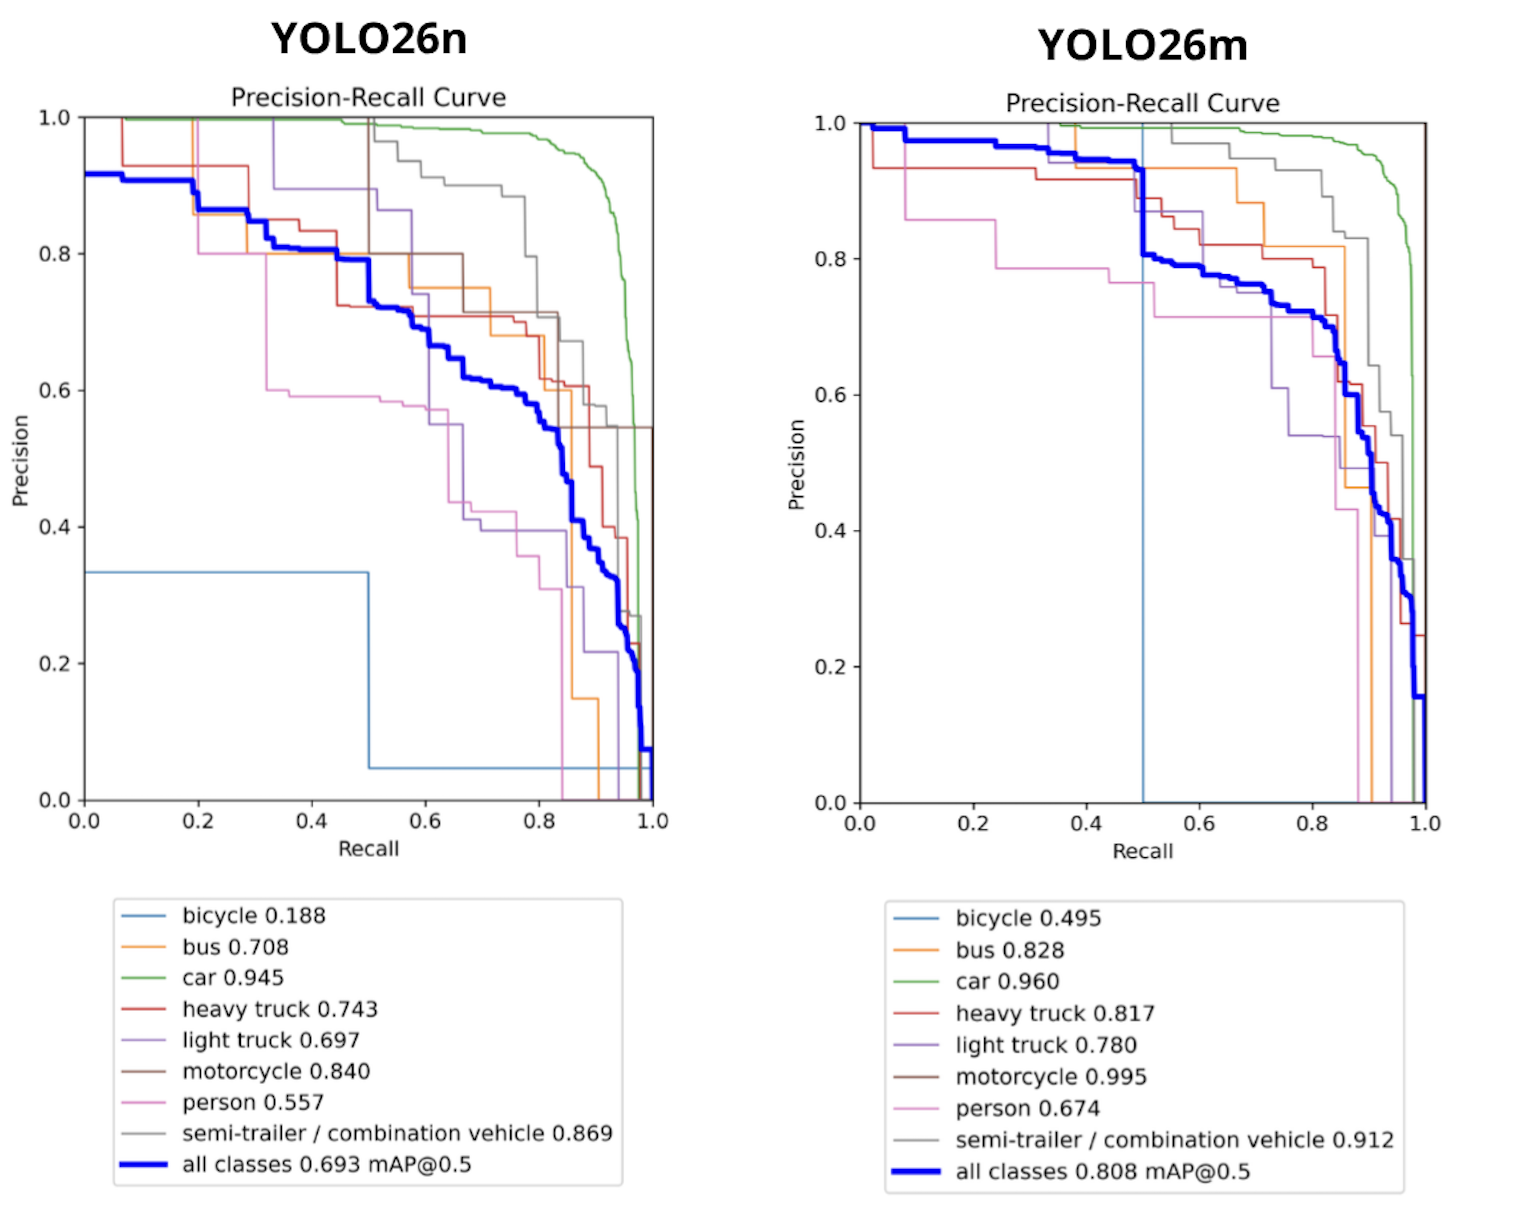
\includegraphics[width=1\linewidth]{project//images//yolo_n_vs_m/PR-curves.png}
    \caption{Precision-Recall curve for all classes for both models. The area under each curve represents the average precision for a specific class.}
    \label{fig:BoxPR_curve}
\end{figure}

The raw counts and row-normalized confusion matrices for the test dataset are presented in \autoref{fig:yolo26n_conf_raw} and \autoref{fig:yolo26n_conf_norm} (YOLO26n) as well as \autoref{fig:yolo26m_conf_raw} and \autoref{fig:yolo26m_conf_norm} (YOLO26m). Both models exhibit strong diagonal values, indicating high recall across most classes. The 'Car' class, in particular, demonstrates exceptional prediction reliability (0.87 for YOLO26n and 0.92 for YOLO26m). Furthermore, the YOLO26m variant shows a marked improvement in recall for the 'Person' class (0.69 vs.\ 0.48) and the 'Semi-trailer' class (0.81 vs.\ 0.72), indicating better detection in these categories compared to the nano model.

Both models exhibit some confusion with the background. As "background" is not a defined object class, it has no true positives. False negatives against the background represent annotated objects that the model failed to detect, while false positives represent regions where the model incorrectly predicted an object where none was annotated.
The YOLO26n model, for example, produced 77 false negatives for cars and 41 false positives. The YOLO26m model shows a similar pattern.

\begin{figure}[H]
    \centering
    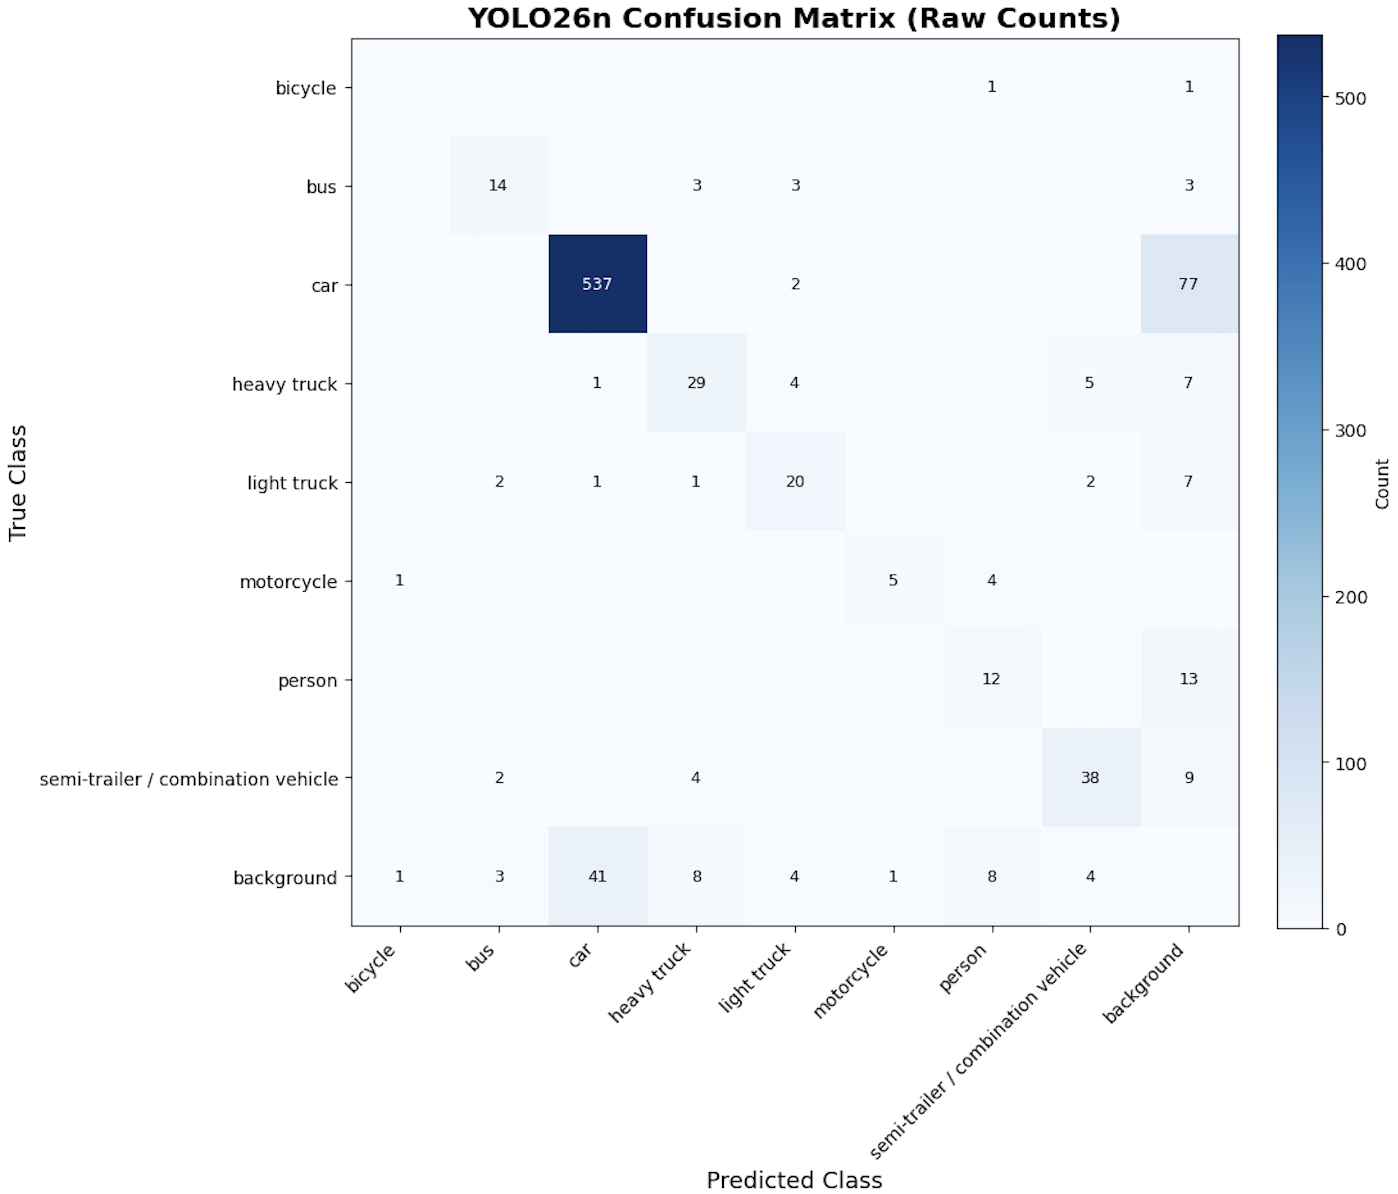
\includegraphics[width=1\linewidth]{project//images//yolo_test/yolo26n_conf_raw.png}
    \caption{YOLO26n Confusion Matrix (Raw Counts)}
    \label{fig:yolo26n_conf_raw}
\end{figure}
\begin{figure}[H]
    \centering
    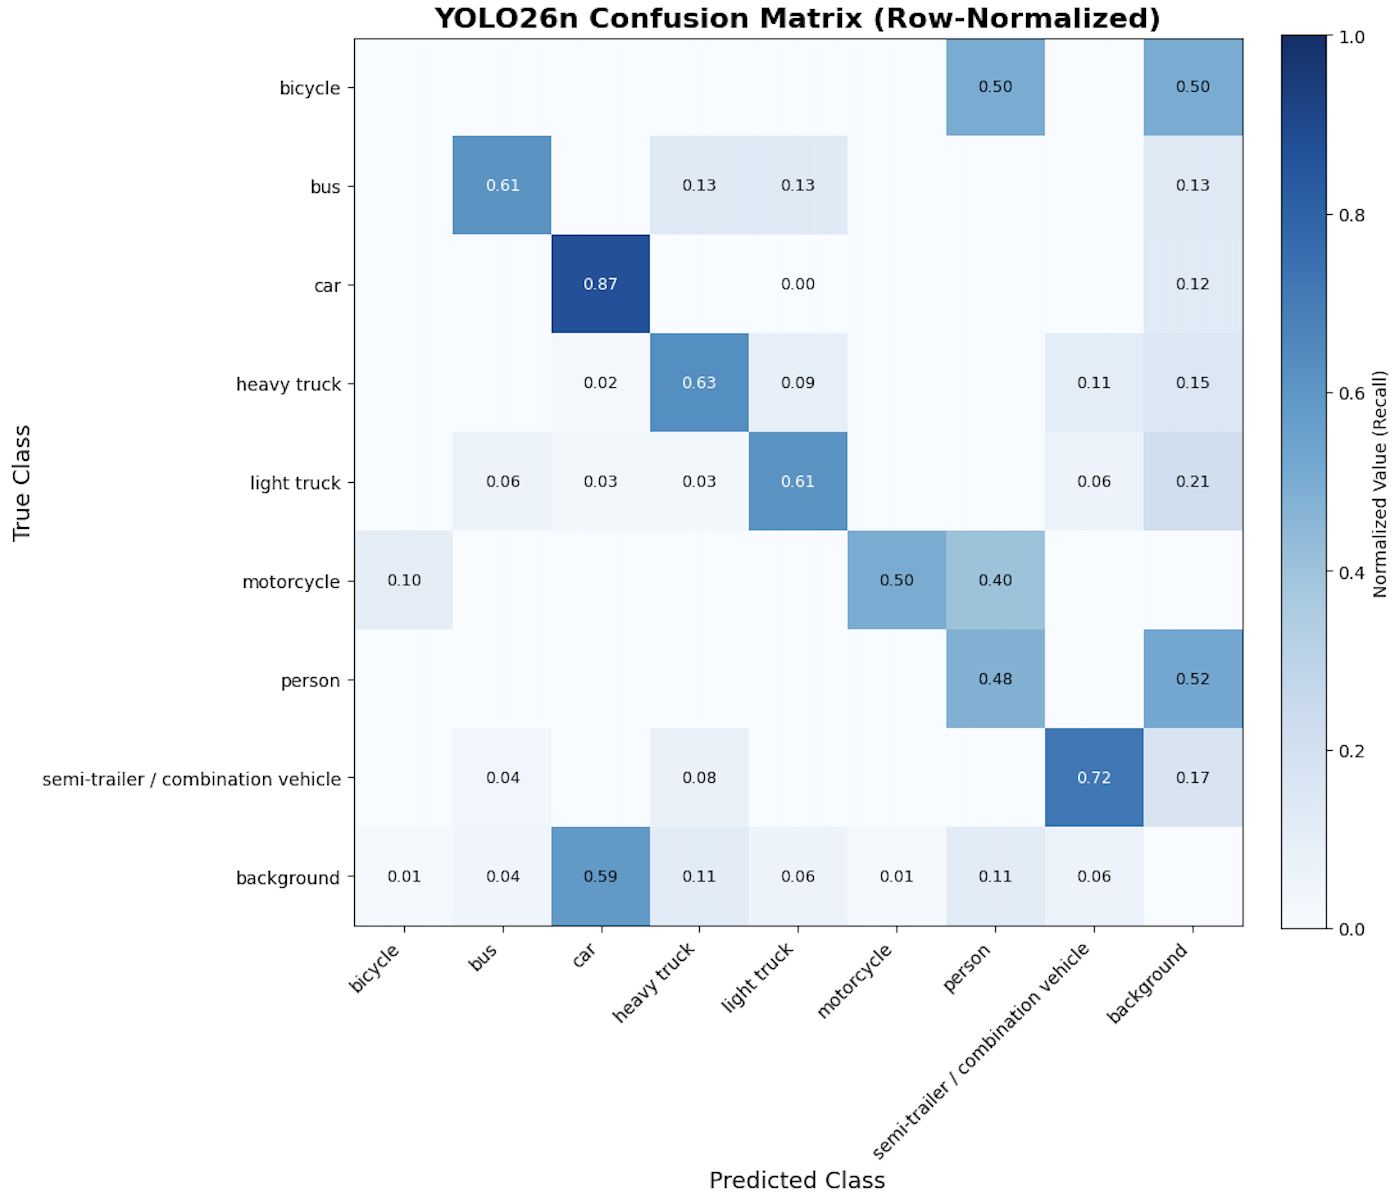
\includegraphics[width=1\linewidth]{project//images//yolo_test/yolo26n_conf_norm.png}
    \caption{YOLO26n Confusion Matrix (Row-Normalized)}
    \label{fig:yolo26n_conf_norm}
\end{figure}
\begin{figure}[H]
    \centering
    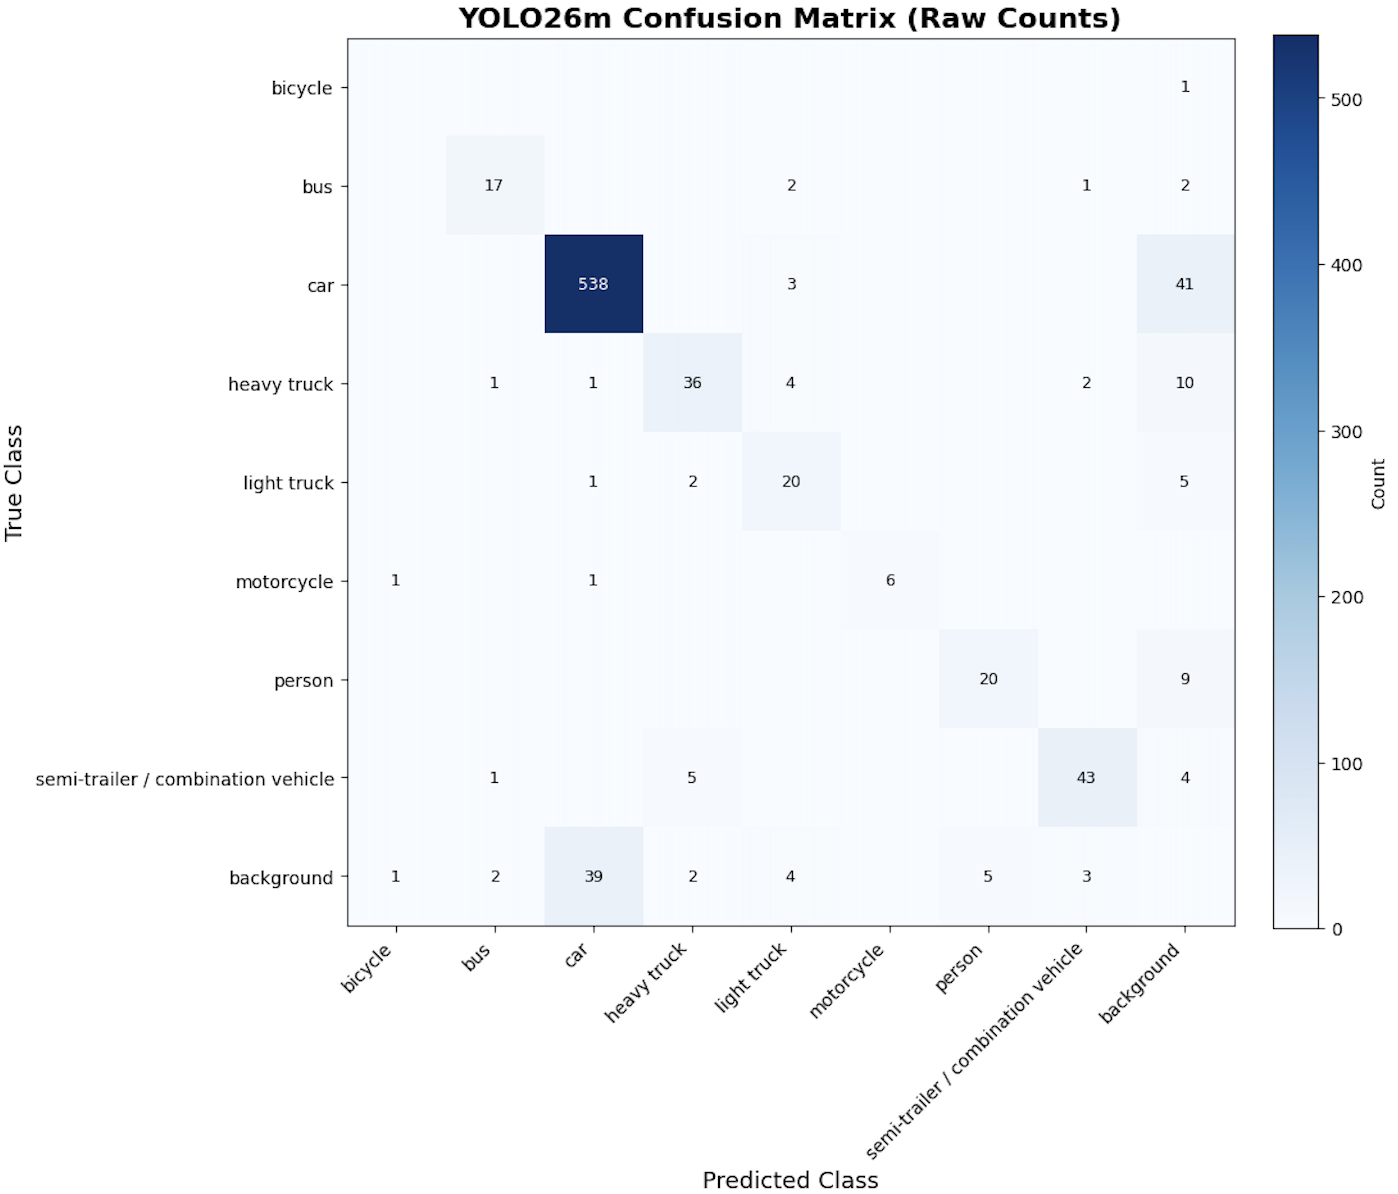
\includegraphics[width=1\linewidth]{project//images//yolo_test/yolo26m_conf_raw.png}
    \caption{YOLO26m Confusion Matrix (Raw Counts)}
    \label{fig:yolo26m_conf_raw}
\end{figure}
\begin{figure}[H]
    \centering
    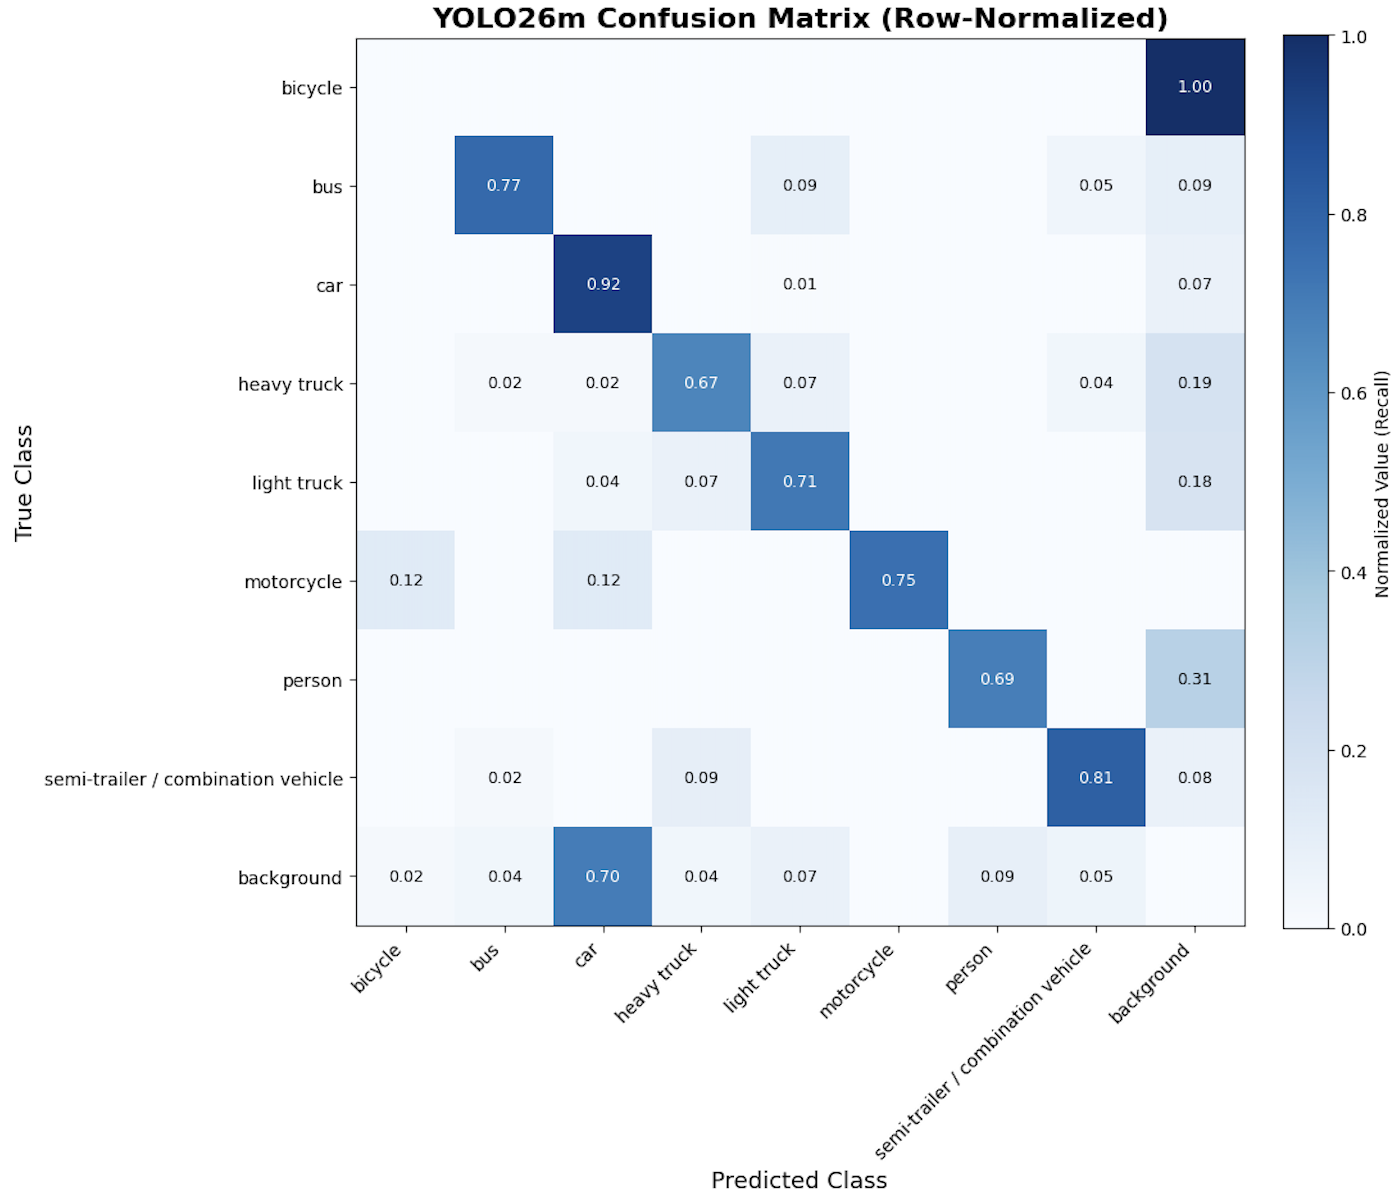
\includegraphics[width=1\linewidth]{project//images//yolo_test/yolo26m_conf_norm.png}
    \caption{YOLO26m Confusion Matrix (Row-Normalized)}
    \label{fig:yolo26m_conf_norm}
\end{figure}


\section{Tracking Results}
\label{sec:tracking_results}

This section presents the results for the tracking pipeline, which associates detections into vehicle trajectories and aggregates them into Origin--Destination (O--D) movements using gate-zone logic. The evaluation covers how different model-tracker combinations reproduce a manually annotated ground-truth O--D matrix, how the pipeline performs under night-time low-light conditions with dedicated preprocessing, and the runtime and tracking stability characteristics relevant to operational deployment. These results form the basis for evaluating the second research question on how different model configurations perform under varying lightning conditions.

\subsection{Daytime Tracking Performance}
\label{subsec:daytime_tracking}

The daytime tracking evaluation used a 15-minute video segment recorded under daylight conditions at the Fv587 Haukeland intersection. Six model-tracker combinations were tested: YOLO26n and YOLO26m paired with three tracking algorithms (ByteTrack, default BoT-SORT, and a custom Day BoT-SORT). For each combination, the predicted O--D matrix was compared against manually annotated ground truth using Sum MAE (mean error across routes), Cell MAE (mean error per O--D cell), total count error, absolute percentage error, and number of perfectly matched routes.

\subsubsection{Comparative Analysis: All Daytime Model-Tracker Combinations}

\autoref{tab:od_daytime_all} summarises the performance of all six model-tracker combinations evaluated on the 15-minute daytime segment. YOLO26m consistently outperforms YOLO26n across all three tracker variants, achieving lower Cell MAE and Sum MAE. Within the YOLO26m configurations, tracker selection has minimal effect on accuracy: Day BoT-SORT achieves the lowest Cell MAE (0.048), followed by BoT-SORT and Bytetrack (both 0.143). The YOLO26n configurations show greater variability, with Cell MAE ranging from 0.167 to 0.310. Bytetrack is the fastest
tracker across both models, processing the 15-minute segment in 267/360 seconds, while Day BoT-SORT with YOLO26m is the slowest at 488 seconds. Person detection at the pedestrian crossing shows differences: YOLO26n fails to detect any persons (100\% error across all trackers), while YOLO26m with Day BoT-SORT perfectly detects all 3 persons present. Other YOLO26m configurations overcount persons (predicting 5 instead of 3, resulting in 66.7\% error).

\begin{table}[H]
\centering
\small
\begin{tabular}{l l c c c c c}
\toprule
\textbf{Model} & \textbf{Tracker} & \textbf{Cell MAE} & \textbf{Sum MAE} & \textbf{Total} & \textbf{Err \%} & \textbf{Time (s)} \\
\midrule
YOLO26m & Day BoT-SORT & 0.048 & 0.000 & 238 & 0.0\% & 488 \\
YOLO26m & Bytetrack & 0.143 & 0.000 & 238 & 0.0\% & 360 \\
YOLO26m & BoT-SORT & 0.143 & 0.000 & 238 & 0.0\% & 531 \\
YOLO26n & Bytetrack & 0.167 & 0.500 & 239 & 0.4\% & 267 \\
YOLO26n & BoT-SORT & 0.214 & 0.500 & 239 & 0.4\% & 476 \\
YOLO26n & Day BoT-SORT & 0.310 & 0.833 & 243 & 2.1\% & 416 \\
\bottomrule
\end{tabular}
\caption{Daytime results: all model-tracker combinations (15-minute daylight segment).}
\label{tab:od_daytime_all}
\end{table}



\begin{table}[H]
\centering
\small
\begin{tabular}{l l c c c c}
\toprule
\textbf{Model} & \textbf{Tracker} & \textbf{GT Persons} & \textbf{Predicted} & \textbf{Error} & \textbf{Err \%} \\
\midrule
YOLO26n & Bytetrack & 3 & 0 & -3 & 100.0\% \\
YOLO26n & BoT-SORT & 3 & 0 & -3 & 100.0\% \\
YOLO26n & Day BoT-SORT & 3 & 0 & -3 & 100.0\% \\
YOLO26m & Bytetrack & 3 & 5 & +2 & 66.7\% \\
YOLO26m & BoT-SORT & 3 & 5 & +2 & 66.7\% \\
YOLO26m & Day BoT-SORT & 3 & 3 & 0 & 0.0\% \\
\bottomrule
\end{tabular}
\caption{Daytime person detection results: all model-tracker combinations.}
\label{tab:persons_daytime}
\end{table}

\autoref{fig:daytime_class_composition} shows total detections by class across all model-tracker combinations. The y-axis uses a logarithmic scale to handle the wide range: cars dominate at ~1000 detections, making smaller classes nearly invisible on a linear scale. YOLO26m consistently tracks closer to ground truth across all classes. \autoref{fig:daytime_class_composition_pct} shows the corresponding per-class percentage errors, where YOLO26n exhibits large errors (up to ~100\%) on these rare classes, while YOLO26m stays lower.

\begin{figure}[H]
    \centering
    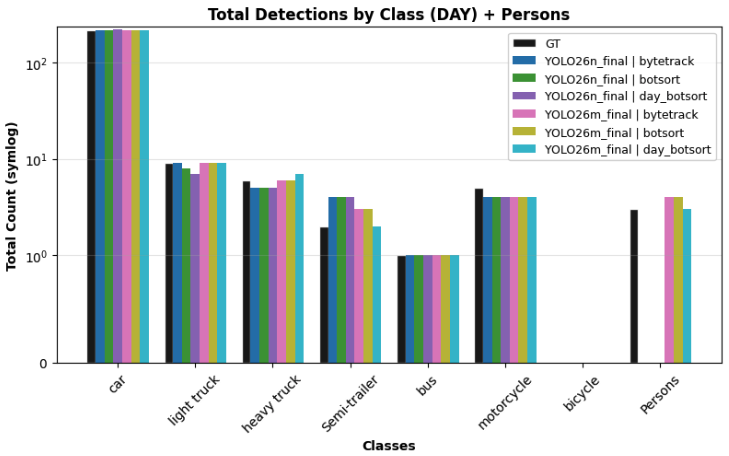
\includegraphics[width=1\linewidth]{project/images/daytime_class_composition_2.png}
    \caption{Predicted vehicle-class composition for each daytime model-tracker combination, compared with ground truth. Total counts (symlog).}
    \label{fig:daytime_class_composition}
\end{figure}

\begin{figure}[H]
    \centering
    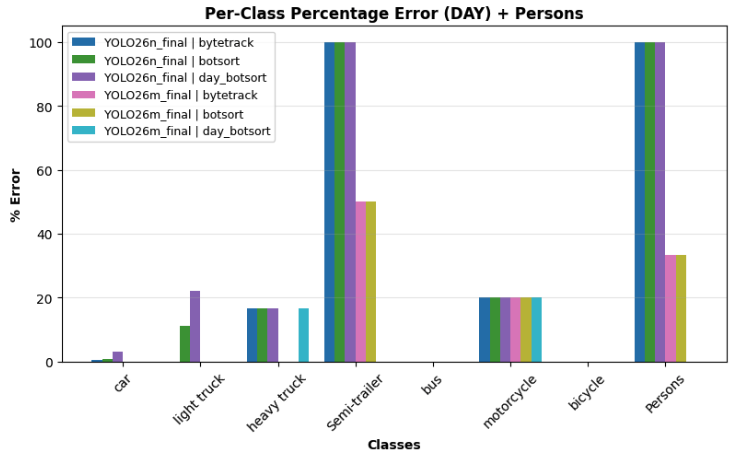
\includegraphics[width=1\linewidth]{project/images/daytime_class_composition_pct.png}
    \caption{Predicted vehicle-class composition for each daytime model-tracker combination, compared with ground truth. Per-class \%-error.}
    \label{fig:daytime_class_composition_pct}
\end{figure}


\subsubsection{Best Daytime Configuration: YOLO26m + Day BoT-SORT}

The detailed O–D prediction matrix and error analysis for YOLO26m + Day BoT-SORT are presented in \autoref{tab:best_day_pred} and \ref{tab:best_day_error}. The configuration accurately captured the dominant traffic movements (S→N: 594 vehicles, N→S: 408 vehicles) with a total undercounting of 10 vehicles (0.9\% error), which is acceptable for operational monitoring. The model maintains consistent accuracy across major routes, with most per-route errors under 5 vehicles. The S→E route shows a 22.2\% overprediction (22 predicted vs 18 ground truth), primarily due to 2 additional motorcycles and 2 additional bicycles. Given that manual traffic counting over a 1-hour period is prone to human error, the small 0.9\% deviation on overall totals suggests the model predictions are reliable for operational monitoring.

Person detection at the pedestrian crossing achieved high accuracy, detecting 6 out of 7 persons (-1 error, 14.3\% error rate).

\begin{table}[H]
\centering
\small
\begin{tabular}{l c c c c c c c c}
\toprule
\textbf{Route} & \textbf{Car} & \textbf{Light} & \textbf{Heavy} & \textbf{Semi-} & \textbf{Bus} & \textbf{Motor-} & \textbf{Bi-} & \textbf{Total} \\
 & & \textbf{Truck} & \textbf{Truck} & \textbf{Trailer} &  & \textbf{cycle} & \textbf{cycle} &  \\
\midrule
S→N & 529 & 19 & 11 & 14 & 3 & 17 & 1 & 594 \\
N→S & 352 & 11 & 11 & 15 & 3 & 14 & 2 & 408 \\
E→S & 18 & 0 & 0 & 0 & 0 & 0 & 0 & 18 \\
E→N & 16 & 1 & 0 & 0 & 0 & 0 & 0 & 17 \\
S→E & 18 & 0 & 0 & 0 & 0 & 3 & 1 & 22 \\
N→E & 10 & 1 & 0 & 0 & 2 & 0 & 0 & 13 \\
\bottomrule
\textbf{Total} & 943 & 32 & 22 & 29 & 8 & 34 & 4 & 1072 \\
\bottomrule
\end{tabular}
\caption{Predicted O–D vehicle counts for YOLO26m + Day BoT-SORT (daytime, 1-hour segment).}
\label{tab:best_day_pred}
\end{table}

\begin{table}[H]
\centering
\small
\begin{tabular}{l c c c c c c c c}
\toprule
\textbf{Route} & \textbf{Car} & \textbf{Light} & \textbf{Heavy} & \textbf{Semi-} & \textbf{Bus} & \textbf{Motor-} & \textbf{Bi-} & \textbf{Total} \\
 & & \textbf{Truck} & \textbf{Truck} & \textbf{Trailer} &  & \textbf{cycle} & \textbf{cycle} &  \\
\midrule
S→N & +6 & +3 & -3 & -1 & 0 & 0 & 0 & +5 \\
N→S & -2 & 0 & 0 & +1 & +1 & +1 & 0 & +1 \\
E→S & 0 & 0 & 0 & 0 & 0 & 0 & 0 & 0 \\
E→N & 0 & +1 & 0 & 0 & 0 & 0 & -1 & 0 \\
S→E & +4 & 0 & 0 & 0 & 0 & +2 & -2 & +4 \\
N→E & 0 & 0 & 0 & 0 & 0 & 0 & 0 & 0 \\
\bottomrule
\textbf{Total} & +8 & +4 & -3 & 0 & +1 & +3 & -3 & +10 \\
\bottomrule
\end{tabular}
\caption{Error analysis (predicted $-$ ground truth; GT total = 1062 vehicles, 0.9\% error).}
\label{tab:best_day_error}
\end{table}


\subsection{Night-Time Tracking Performance}
\label{subsec:nighttime_tracking}

To evaluate robustness under low-light conditions, the pipeline was tested on a 1-hour night-time video segment from the same intersection, captured under artificial street lighting. Night-time evaluation incorporated conservative tracking hyperparameters, as described in Section~\ref{chap:methods}. In addition to the standard tracker configurations, a custom Night BoT-SORT variant was developed specifically for low-light conditions, with tuned hyperparameters to reduce noise-induced fragmentation and improve identity retention under degraded visual input. No pedestrians crossed the road in the nighttime footage, so no results are reported.

\subsubsection{Comparative Analysis: All Night-Time Configurations}

Table~\ref{tab:od_nighttime_all} presents the performance of all six model-tracker combinations evaluated on the night-time segment. YOLO26m + Night BoT-SORT Conservative achieved the best overall performance with a Sum MAE of 0.67 and perfect vehicle count accuracy (0.0\% error). The other YOLO26m configurations showed comparable results, with Sum MAE values of 1.17 and modest 2.3\% deviations in vehicle totals. The YOLO26n configurations exhibited higher Cell MAE (up to 0.40) and Sum MAE (up to 1.83), with one configuration achieving perfect total counts (0.0\% error) while others showed 2.3\% deviations. Despite these differences, all configurations maintained reasonable accuracy under low-light conditions, with the larger YOLO26m model offering more stable class predictions overall.

\begin{table}[H]
\centering
\small
\begin{tabular}{l l c c c c c}
\toprule
\textbf{Model} & \textbf{Tracker} & \textbf{Cell} & \textbf{Sum} & \textbf{Tot} & \textbf{Err} & \textbf{Time} \\
 &  & \textbf{MAE} & \textbf{MAE} &  & \textbf{\%} & \textbf{(s)} \\
\midrule
YOLO26m & Night BoT-SORT Cons. & 0.29 & 0.67 & 132 & 0.0 & 564 \\
YOLO26m & ByteTrack              & 0.31 & 1.17 & 129 & 2.3 & 566 \\
YOLO26m & Night BoT-SORT        & 0.36 & 1.17 & 129 & 2.3 & 568 \\
YOLO26n & Night BoT-SORT Cons. & 0.36 & 1.50 & 131 & 0.8 & 432 \\
YOLO26n & ByteTrack              & 0.40 & 1.83 & 129 & 2.3 & 430 \\
YOLO26n & Night BoT-SORT        & 0.40 & 1.83 & 129 & 2.3 & 430 \\
\bottomrule
\end{tabular}
\caption{Nighttime results: all model-tracker combinations (sorted by Cell MAE, then Sum MAE).}
\label{tab:od_nighttime_all}
\end{table}

\begin{figure}[H]
    \centering
    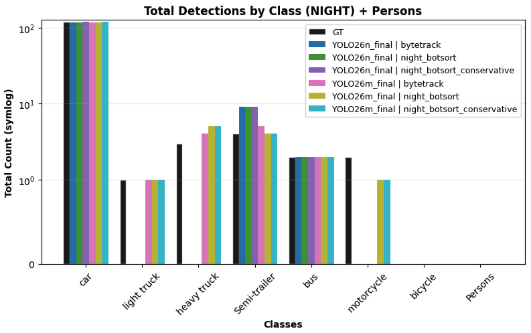
\includegraphics[width=1\linewidth]{project/images/nighttime_class_composition2.png}
    \caption{Predicted vehicle-class composition for night-time model-tracker
    combinations, compared with ground truth. Raw counts (symlog).}
    \label{fig:class_comp_night}
\end{figure}

\begin{figure}[H]
    \centering
    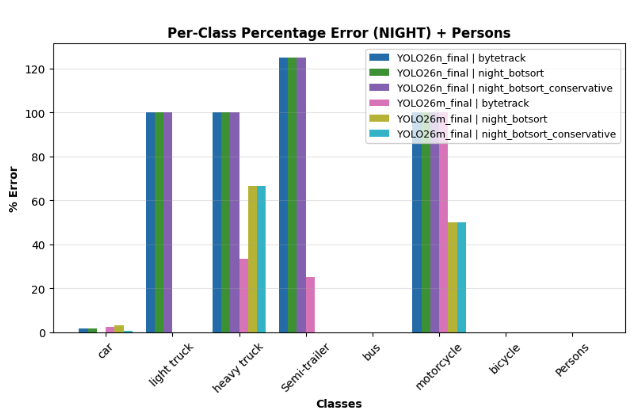
\includegraphics[width=1\linewidth]{project/images/nighttime_class_composition_pct.png}
    \caption{Predicted vehicle-class composition for night-time model-tracker
    combinations, compared with ground truth. Per class \%-error.}
    \label{fig:class_comp_night_pct}
\end{figure}

As shown in Figure~\ref{fig:class_comp_night} and \ref{fig:class_comp_night_pct}, YOLO26m consistently outperforms YOLO26n across all vehicle classes. YOLO26m + Night BoT-SORT Conservative achieves the smallest prediction error on most classes. The exception is the heavy truck class, where ByteTrack performs best. In contrast, YOLO26n configurations exhibit larger errors across classes, particularly misclassifying heavy trucks as semi-trailers and struggling with motorcycle detection.

\subsubsection{Best Night-Time Configuration in Detail: YOLO26m + Night BoT-SORT Conservative}

The YOLO26m + Night BoT-SORT Conservative configuration achieved the best overall performance among all night-time model-tracker combinations, with perfect vehicle count totals (0\% error) and the lowest Sum MAE (0.67). This configuration was developed specifically for low-light conditions and maintains balanced tracking performance across all route segments. The detailed O--D prediction matrix and error analysis are presented in Tables~\ref{tab:od_nighttime_best} and~\ref{tab:od_nighttime_error}.

\begin{table}[H]
\centering
\small
\begin{tabular}{l c c c c c c c c}
\toprule
\textbf{Route} & \textbf{Car} & \textbf{Light} & \textbf{Heavy} & \textbf{Semi-} & \textbf{Bus} & \textbf{Motor-} & \textbf{Bi-} & \textbf{Total} \\
 & & \textbf{Truck} & \textbf{Truck} & \textbf{Trailer} &  & \textbf{cycle} & \textbf{cycle} &  \\
\midrule
S$\to$N & 60 & 0 & 5 & 2 & 1 & 0 & 0 & 68 \\
N$\to$S & 53 & 1 & 0 & 2 & 1 & 1 & 0 & 58 \\
E$\to$S & 2  & 0 & 0 & 0 & 0 & 0 & 0 & 2  \\
E$\to$N & 2  & 0 & 0 & 0 & 0 & 0 & 0 & 2  \\
S$\to$E & 2  & 0 & 0 & 0 & 0 & 0 & 0 & 2  \\
N$\to$E & 0  & 0 & 0 & 0 & 0 & 0 & 0 & 0  \\
\bottomrule
\textbf{Total} & 119 & 1 & 5 & 4 & 2 & 1 & 0 & 132 \\
\bottomrule
\end{tabular}
\caption{Predicted O--D vehicle counts for YOLO26m + Night BoT-SORT Conservative (night-time test).}
\label{tab:od_nighttime_best}
\end{table}

\begin{table}[H]
\centering
\small
\begin{tabular}{l c c c c c c c c}
\toprule
\textbf{Route} & \textbf{Car} & \textbf{Light} & \textbf{Heavy} & \textbf{Semi-} & \textbf{Bus} & \textbf{Motor-} & \textbf{Bi-} & \textbf{Total} \\
 & & \textbf{Truck} & \textbf{Truck} & \textbf{Trailer} &  & \textbf{cycle} & \textbf{cycle} &  \\
\midrule
S$\to$N & 0 & 0 & $+4$ & $-2$ & 0 & 0 & 0 & $+2$ \\
N$\to$S & $-1$ & 0 & $-2$ & $+2$ & 0 & $-1$ & 0 & $-2$ \\
E$\to$S & 0 & 0 & 0 & 0 & 0 & 0 & 0 & 0 \\
E$\to$N & 0 & 0 & 0 & 0 & 0 & 0 & 0 & 0 \\
S$\to$E & 0 & 0 & 0 & 0 & 0 & 0 & 0 & 0 \\
N$\to$E & 0 & 0 & 0 & 0 & 0 & 0 & 0 & 0 \\
\bottomrule
\textbf{Total} & $-1$ & 0 & $+2$ & 0 & 0 & $-1$ & 0 & 0 \\
\bottomrule
\end{tabular}
\caption{Error analysis (predicted $-$ ground truth; GT total = 132 vehicles, 0.0\% error) for YOLO26m + Night BoT-SORT Conservative.}
\label{tab:od_nighttime_error}
\end{table}

\subsection{Adaptive Dual-Tracker Configuration: Real-Time Lighting Conditions}

To enable continuous 24/7 operation without manual intervention, an adaptive dual-tracker system was implemented that automatically switches between the optimal day-time and night-time configurations based on real-time lighting conditions. The system monitors video saturation levels and applies a grayscale filter when saturation drops below a threshold, triggering an automatic switch from YOLO26m + ByteTrack (daytime) to YOLO26m + Night BoT-SORT Conservative (night-time). This approach leverages the strengths of each configuration while maintaining seamless transitions across lighting variations.

To evaluate this adaptive strategy, a 10-minute twilight sequence was analysed, covering a transition from daylight to night-time conditions. The results are used to assess the third research question concerning the ability of a vision-based traffic monitoring system to operate autonomously over time without manual intervention. As shown in Tables~\ref{tab:od_twilight_best} and~\ref{tab:od_twilight_error}, the dual-tracker configuration achieved perfect accuracy across all routes and vehicle classes, with zero errors (0.0\% absolute percentage error) and zero Sum MAE. All six routes were predicted with exact precision, demonstrating that the adaptive switching mechanism successfully maintains optimal performance across dynamic lighting conditions.



\begin{table}[H]
\centering
\small
\begin{tabular}{l c c c c c c c c}
\toprule
\textbf{Route} & \textbf{Car} & \textbf{Light} & \textbf{Heavy} & \textbf{Semi-} & \textbf{Bus} & \textbf{Motor-} & \textbf{Bi-} & \textbf{Total} \\
 & & \textbf{Truck} & \textbf{Truck} & \textbf{Trailer} &  & \textbf{cycle} & \textbf{cycle} &  \\
\midrule
S$\to$N & 16 & 0 & 0 & 0 & 0 & 0 & 0 & 16 \\
N$\to$S & 10 & 0 & 0 & 0 & 1 & 0 & 1 & 12 \\
E$\to$S & 0  & 0 & 0 & 0 & 0 & 0 & 0 & 0  \\
E$\to$N & 1  & 0 & 0 & 0 & 0 & 0 & 0 & 1  \\
S$\to$E & 1  & 0 & 0 & 0 & 0 & 0 & 0 & 1  \\
N$\to$E & 0  & 0 & 0 & 0 & 0 & 0 & 0 & 0  \\
\bottomrule
\textbf{Total} & 28 & 0 & 0 & 0 & 1 & 0 & 1 & 30 \\
\bottomrule
\end{tabular}
\caption{Predicted O--D vehicle counts for adaptive dual-tracker system (twilight segment, 10 minutes).}
\label{tab:od_twilight_best}
\end{table}

\begin{table}[H]
\centering
\small
\begin{tabular}{l c c c c c c c c}
\toprule
\textbf{Route} & \textbf{Car} & \textbf{Light} & \textbf{Heavy} & \textbf{Semi-} & \textbf{Bus} & \textbf{Motor-} & \textbf{Bi-} & \textbf{Total} \\
 & & \textbf{Truck} & \textbf{Truck} & \textbf{Trailer} &  & \textbf{cycle} & \textbf{cycle} &  \\
\midrule
S$\to$N & 0 & 0 & 0 & 0 & 0 & 0 & 0 & 0 \\
N$\to$S & 0 & 0 & 0 & 0 & 0 & 0 & 0 & 0 \\
E$\to$S & 0 & 0 & 0 & 0 & 0 & 0 & 0 & 0 \\
E$\to$N & 0 & 0 & 0 & 0 & 0 & 0 & 0 & 0 \\
S$\to$E & 0 & 0 & 0 & 0 & 0 & 0 & 0 & 0 \\
N$\to$E & 0 & 0 & 0 & 0 & 0 & 0 & 0 & 0 \\
\bottomrule
\textbf{Total} & 0 & 0 & 0 & 0 & 0 & 0 & 0 & 0 \\
\bottomrule
\end{tabular}
\caption{Error analysis (predicted $-$ ground truth; GT total = 29 vehicles, 0\% error) for adaptive dual-tracker system.}
\label{tab:od_twilight_error}
\end{table}



\begin{figure}[H]
    \centering
    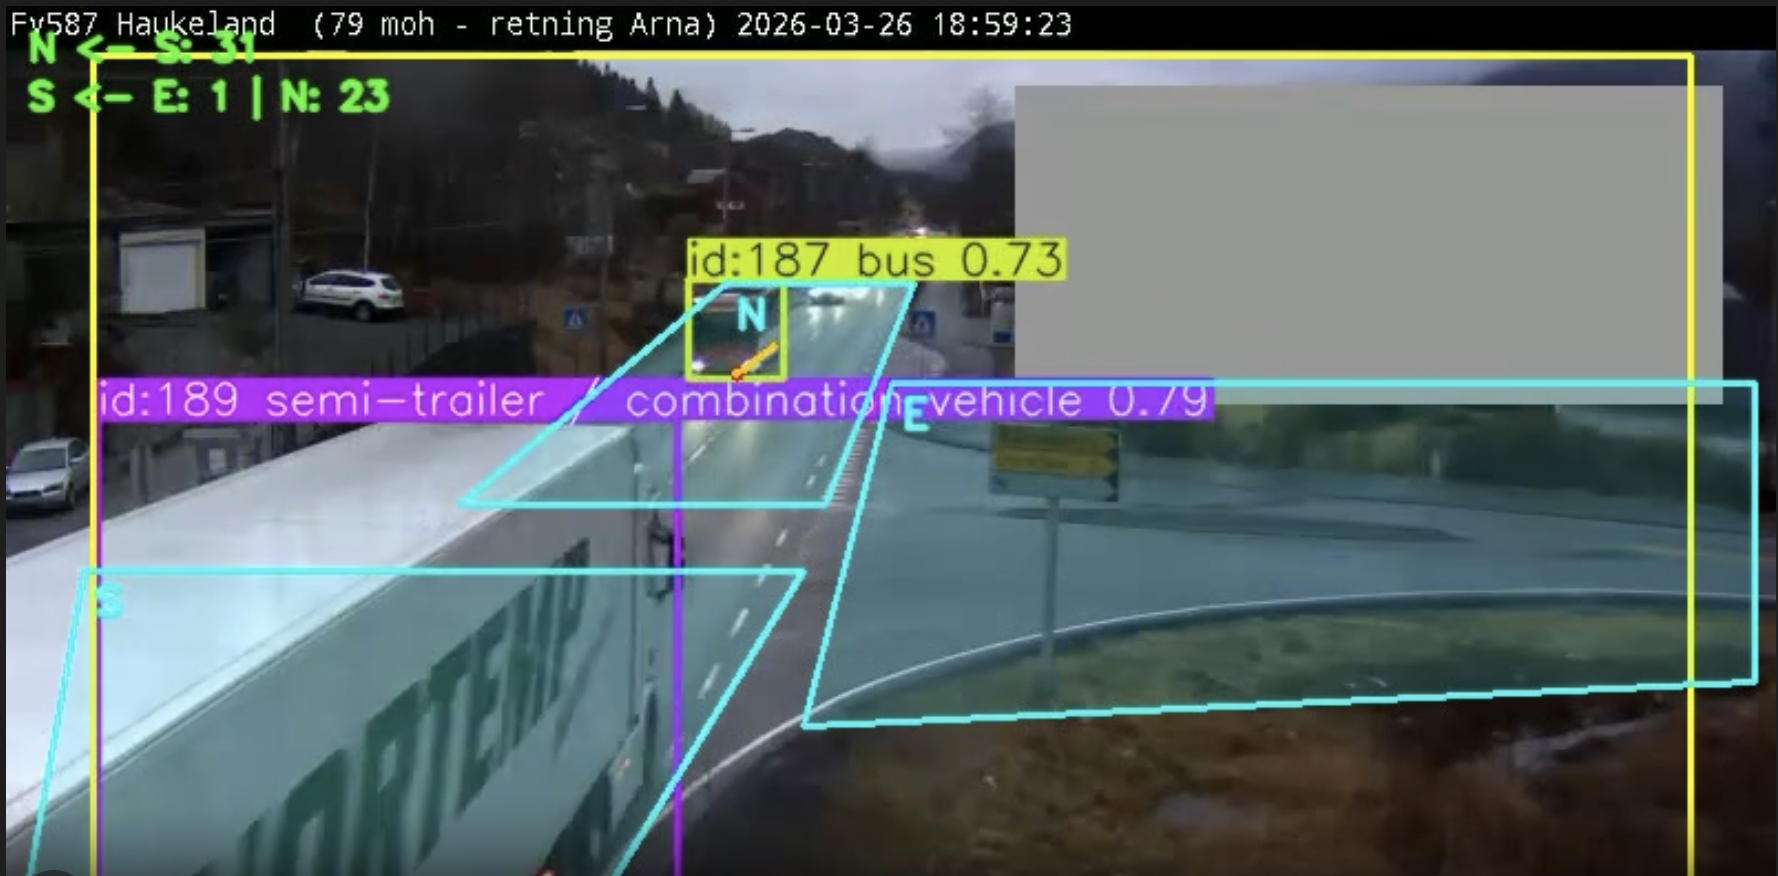
\includegraphics[width=0.75\linewidth]{project/images/occlution_before.png}
    \vspace{4pt}
    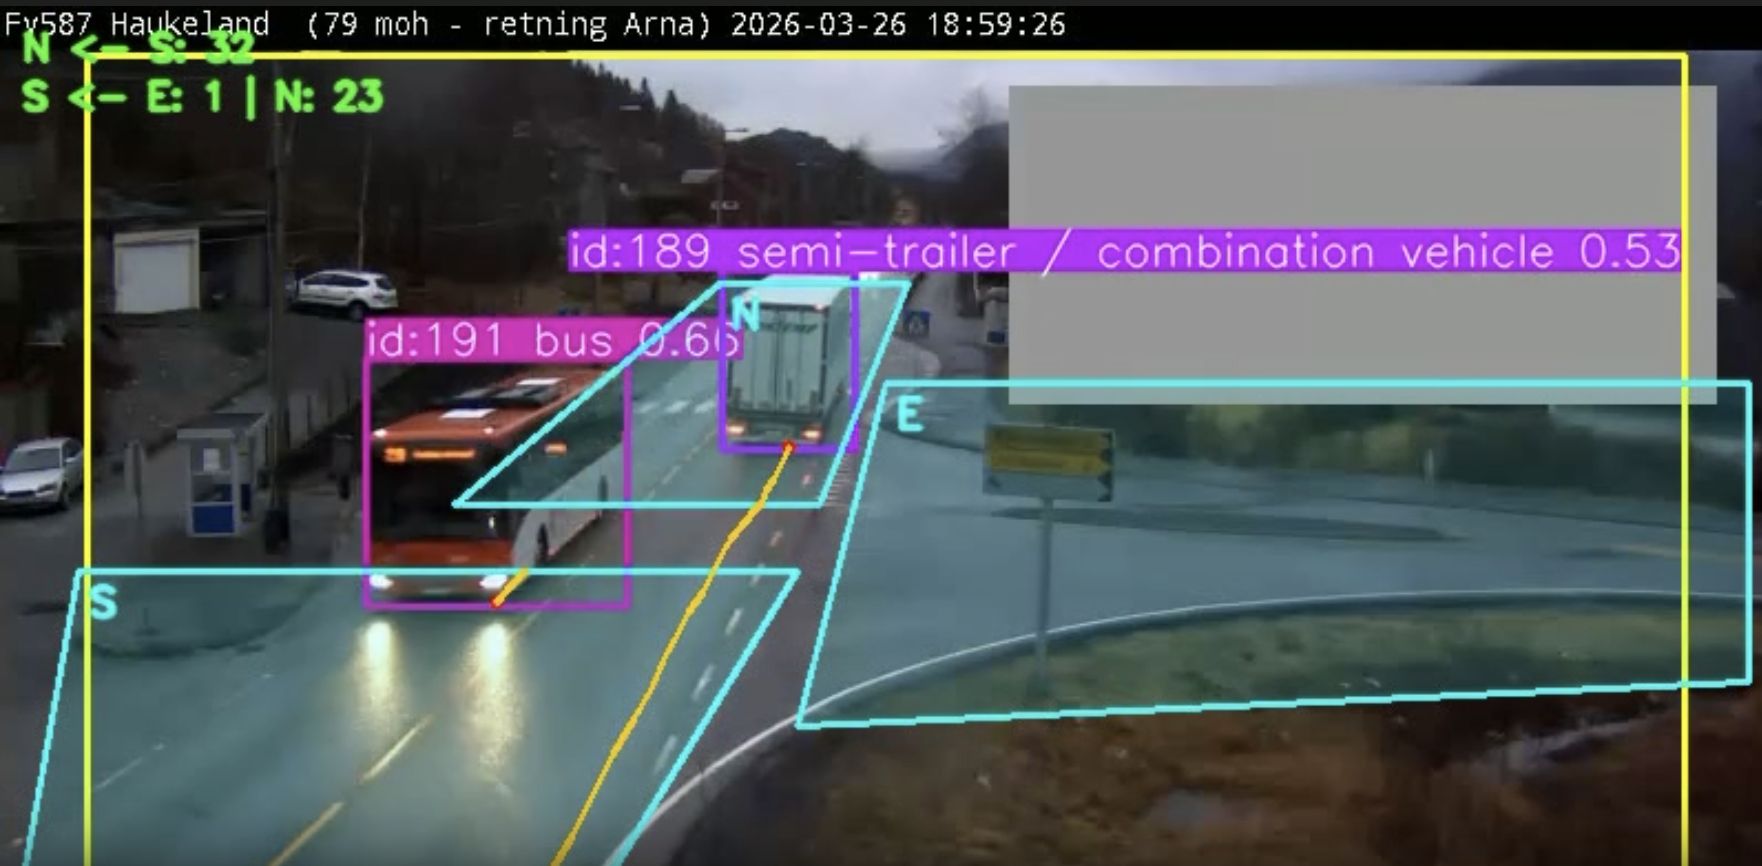
\includegraphics[width=0.75\linewidth]{project/images/occlution_after.png}
    \caption[Occlusion event during live deployment]{Occlusion event during live deployment: the bus (ID:187) is fully obscured
        by a semi-trailer (top), and re-emerges with a new track ID:191 (bottom).}
    \label{fig:tracking_occlusion}
\end{figure}


